\documentclass[20pt,,margin=1in,innermargin=-4.5in,blockverticalspace=-0.25in]{tikzposter}
\geometry{paperwidth=42in,paperheight=32.5in}
\usepackage[utf8]{inputenc}
\usepackage{amsmath}
\usepackage{amsfonts}
\usepackage{amsthm}
\usepackage{amssymb}
\usepackage{mathrsfs}
\usepackage{graphicx}
\usepackage{adjustbox}
\usepackage{enumitem}
\usepackage[backend=biber,style=numeric]{biblatex}
\usepackage{SUtheme}
\usepackage{mathtools}
\usepackage{bm}
\usepackage{bbm}

\usepackage{mwe} % for placeholder images
% notes
\usepackage[color=pink]{todonotes}
\usepackage{marginnote}
\let\marginpar\marginnote

\addbibresource{refs.bib}

% set theme parameters
\tikzposterlatexaffectionproofoff
\usetheme{SUTheme}
\usecolorstyle{SUStyle}
\usetitlestyle{Filled}

\usepackage[scaled]{helvet}
\renewcommand\familydefault{\sfdefault} 
\usepackage[T1]{fontenc}
% figure support
\usepackage{import}
\usepackage{xifthen}
\usepackage{pdfpages}
\usepackage{transparent}
\newcommand{\incfig}[1]{%
	\def\svgwidth{0.35\columnwidth}
	\import{./Figures/}{#1.pdf_tex}
}

\title{Using Graph Neural Network to Solve the Traveling Salesman Problem}
\author{Pingbang Hu, Jonathan Moore, Yi Zhou, Shubham Kumar Pandey, Anuraag Ramesh}
\institute{University of Michigan}
\titlegraphic{
\includegraphics[width=0.06\textwidth]{Figures/U-M_Logo-Hex.png}}

% begin document
\begin{document}
\maketitle
\centering
\begin{columns}
	\column{0.3}
	\block{Abstract}{
		\textbf{Graph neural network} is a rising concept in machine learning that has demonstrated significant potential in many areas.
		Our project aims to further explore this potential by applying it to the classic \textbf{Traveling Salesman Problem (TSP)}.
		We explore a novel concept called \textbf{imitation learning}, which is a special type of \textbf{reinforcement learning}.

		The former works focuses on fixed size training where the problem size is about \(500\) hundreds of constraints with \(1000\) of
		variables. In this work, we focus on generalization ability instead. Specifically, we train on TSP with \(10\) and \(15\) nodes, which
		translate into an \textbf{Integer Linear Programming (ILP)} with hundreds of variables and several hundreds of constraints. Then, we test
		on TSP instances with more nodes and see the generalization ability of this novel approach.
	}
	\block{The Basics of GNN}{
		\textbf{A graph neural network (GNN)} is a class of neural network for processing data best represented by graph structures.
		They were popularized by their use in supervised learning on properties of various molecules from the natural of this task: 3d graph
		structure.

		\par Since their inception, variants of the message passing neural network (MPNN) framework have been proposed. These models optimize
		GNNs for use on larger graphs and apply them to domains such as social networks, citation networks, and online communities. GNNs have
		also been relatively successful in various NP-hard combinatorial problems, automated planning and path-planning areas due to the
		inherent graph structure of data.
		\begin{center}
			\begin{minipage}{0.45\linewidth}
				\centering
				\begin{tikzfigure}
					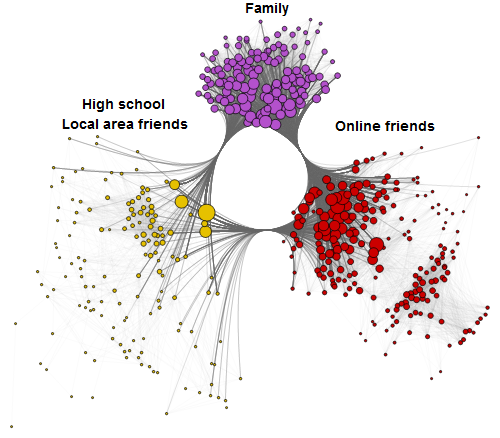
\includegraphics[width=13.6cm]{Figures/GNN_APP.png}
				\end{tikzfigure}%
			\end{minipage}\hfill
			\begin{minipage}{0.55\linewidth}
				\centering
				\begin{tikzfigure}
					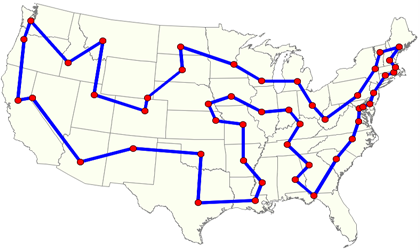
\includegraphics[width=14cm]{Figures/TSP.png}
				\end{tikzfigure}%
			\end{minipage}
		\end{center}
	}

	% NEW COLUMN
	%\column{0.36}
	\block{Problem Formulation}{
		\textbf{The classical TSP} is given in a very simple form: \emph{Given \(n\) nodes with their coordinates, find the closed tour which
			goes through all the nodes with the shortest length.}

		One way to formulate TSP is to model which by \textbf{Integer Linear Programming (ILP)}. Given an undirected weighted graph \(\mathcal{G} = (\mathcal{E}, \mathcal{V})\), we label the
		nodes with numbers \(1, \ldots, n\) and define
		\[
			x_{ij}\coloneqq \begin{dcases}
				1, & \text{if }(i, j)\in \mathcal{E}^\prime                       \\
				0, & \text{if } (i, j)\in \mathcal{E}\setminus\mathcal{E}^\prime,
			\end{dcases}
		\]
		where \(\mathcal{E}^\prime\subset \mathcal{E}\) is a variable which can be viewed as a compact representation of all variables \(x_{ij}\).
		This means that \(x_{ij}\) acts like an \textbf{indicator} variable, it's \(1\) if it's in the optimal tour,
		\(0\) otherwise. We denote the weight on edge \((i, j)\) by \(c_{ij}\), then for a TSP problem instance, we can formulate the problem
		by so-called \textbf{Miller–Tucker–Zemlin formulation}\cite{MTZ-formulation}.

		One way to solve an ILP is to first \textbf{relax} the integrality constraints by letting \(x_{ij}\in[0, 1]\). Then, we
		can divide the original relaxed LP into two sub-problems by \textbf{splitting the feasible region} according to \textbf{a chosen variable}
	}
	% NEW COLUMN
	\column{0.4}
	\block{}{
		that violates integrality constraints in the current relaxed LP solution \(\bm{x}^\ast\), say \(\bm{x}^\ast _i\), then
		\[
			\bm{x}_{i} \leq \left\lfloor \bm{x}_{i}^\ast \right\rfloor\lor \bm{x}_{i} \geq \left\lceil \bm{x}_{i}^\ast \right\rceil,\qquad \exists i\leq p\mid \bm{x}_{i} ^\ast \notin \mathbb{\MakeUppercase{z}}.
		\]
		are two additional constraints in two sub-problems respectively. This gives us a recursive algorithm called \textbf{Branch and Bound}\cite{B&B.ch7}.
		Note that a good branching decision can reduce the solving time significantly, hence, our plan is simple, we want to solve TSP by branch and bound
		and learn how to branch.

		This is a sequential decision problem, hence, we naturally model this as a \textbf{Markov Decision Process (MDP)} problem\cite{howard1960dynamic}.
	}
	\block{Learning Pipeline}{
	\textbf{Our learning pipeline} is as follows. We first create some random TSP instances, and turn it into ILP. Then, we use imitation
	learning\cite{GasseCFCL19} to learn how to choose the \textbf{branching target} at each branching.

	\begin{tikzfigure}
		\centering
		\incfig{pipeline}
	\end{tikzfigure}
	\textbf{Specifically}, we will pass TSP instances to \texttt{SCIP}, which is a modern SOTA MILP (Mixed Integer Linear Programming) solver, to get all
	the solving states in order to solve MDP problem. The modern solver usually use mixed branching strategy to balance the running
	time, and a well-known costly but strong strategy is called \textbf{strong branching}, and in order to learn the strongest branching strategy, we make
	\texttt{SCIP} to use strong branch with probability a half. This learning process is called \textbf{imitation learning}, or \textbf{behavioral
		cloning}\cite{Efficient-Training-of-artificial-Neural-Networks-for-Autonomous-Navigation}.

	Mathematically, we first run the SOTA solver \texttt{SCIP} to get state-action pairs \(\mathcal{\MakeUppercase{d}} = \left\{(s_{i} , \bm{a} _{i} ^\ast)\right\}_{i = 1}^N\),
	where the states is the solver's branching strategy, and the action set contains what variables we can branch on.


	To learn the policy \(\widetilde{\pi} ^\ast\), we minimize the cross-entropy loss between our branching prediction and the solver's branching choice:
	\[
		\mathcal{\MakeUppercase{l}} (\theta ) = - \frac{1}{N}\sum\limits_{(\bm{s}, \bm{a}^\ast)\in \mathcal{\MakeUppercase{d}} }\log \widetilde{\pi}_\theta (\bm{a} ^\ast \mid \bm{s} ).
	\]

	After learning, we evaluate our model on TSP instances with various sizes to see the generalization ability. Specifically, we use
	Ecole\cite{prouvost2020ecole} to do the evaluation. We configure \texttt{SCIP} to its default strategy and compare the result to our learned branching
	strategy by looking at the time needed to solve this particular TSP instance.
	}
	\column{0.3}
	\block{Experimental Results}{
		\todo[inline]{Wait for the evaluation result}
	}

	\block{Conclusion}{
		Unlike other works which focuses on just to solve TSP approximately, we focus on generalization ability of solving TSP \textbf{exactly}.

		With limited computation power and training on small size instances, our result shows a promising performance on generalization ability of branch, which is a hard
		combinatorial optimization problem and typically hard to generalize.

		\textbf{The significance} of our works is pretty straightforward: We're now confidence to generalize on larger instances by combining various machine learning techniques
		like standard reinforcement learning, deep learning, transformer, etc. This is promising since our result shows that we can fit small instances while
		keep the generalization ability.
		\todo[inline]{discuss}
	}

	\block{Future Work}{
		Due to computational limitation, we can't train on larger instances. One may further generalize our work by training on larger instances, for instance, TSP50.

		On the other hand, our work should be easy to reproduce and be combined with various of standard reinforcement technique to further fine-tuned our trained model.
	}

	% \block{References}{
	% 	\vspace{-1em}
	% 	\begin{footnotesize}
	% 		\printbibliography[heading=none]
	% 	\end{footnotesize}
	% }
\end{columns}
\end{document}
